
\subsection{Pago de jugadas y premios}

Se explicaran aqui con detalle como se refleja el pago de apuestas en el modelo propuesto (Modelo de Clases)\\
\textbf{NOTA: } Esta seccion esta dirigida a solo a lectores con conocimientos de modelo de clases conceptuales y OCL. 

\newpage

\subsection{Registracion y Ingreso al casino online y modificacion de saldo}

\subsubsection{Registracion}
Segun lo acordado, la registracion de los usuarios de hace por fuera del sistema informatico del casino online. Explicaremos como esperamos que interactuen los agentes externos para que el sistema posea la lista actualizada de usuarios registrados. Para ello usaremos el Diagrama de Activdades\footnote{Diagrama de Actividades: Grafico que representa el flujo de actividades. Las cajas representan actividades y las flechas repersentan secuencialidad y los rombos representan decisiones} ``Registracion''. Ver Figura: \ref{fig:daReg}

\begin{figure}[h!]
	\centering
		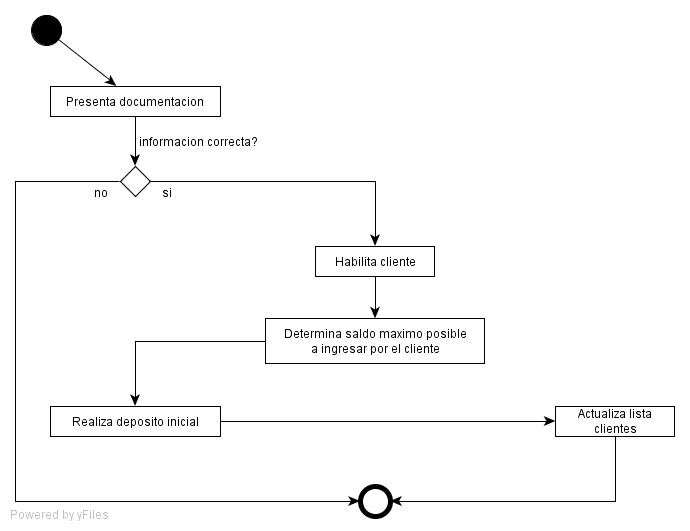
\includegraphics[scale=0.5]{img/daRegistracion.png}
	\caption{Diagrama de actividades Registracion\label{fig:daReg}}
\end{figure}

\textcolor{red}{falta nombre de responsables}

Cabe aclarar que el cliente podra comenzar a jugar en el casino recien cuando el casino se vuelva a abrir

\subsubsection{Modificacion de saldo}

Una vez registrado un cliente puede ingresar y retirar dinero real, dicha operacion solo podra realizarse mistras el casino permanece cerrado.
Explicaremos esta operatoria con un diagrama de actividades. Ver Figura: \ref{fig:modSaldo}

\begin{figure}[h!]
	\centering
		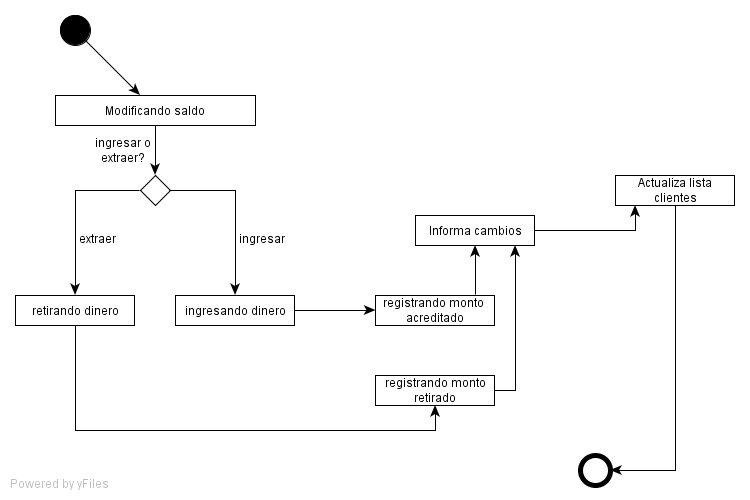
\includegraphics[scale=0.5]{img/clienteModSaldo.png}
	\caption{Diagrama de actividades Modificacion de Saldo\label{fig:modSaldo}}
\end{figure}

\textcolor{red}{falta nombre de responsables}

\subsubsection{Ingreso y egreso del casino}

La forma en que un cliente ingresa o egresa del casino esta explicado en los casos de uso: \textcolor{red}{nombres de CU y referencia}

\subsection{Administracion del Casino}

\subsubsection{Apertura del casino}

En el momento de la apertura del casino es podible realizar configuraciones distintos aspectos:
\begin{itemize}
	\item Configuracion de valores de fichas
	\item Asignacion de probablilidades
	\item valores minimos para la entrega de premios
\end{itemize}

Dicha interaccion con el sistema esta explicada en el caso de uso: \textcolor{red}{falta nombre CU y referencia}

\subsubsection{Clausura del casino}

La operatioria de cerrar el casino no es muy complicada, pero tiene una salvedad. No es posible cerrar el casino si hay jugadores dentro del casino

Dicha interaccion con el sistema esta explicada en el caso de uso: \textcolor{red}{falta nombre CU y referencia}

\begin{framed}

\depto Con esta maquina de estados finitos (FSM) Mostramos que nos comprometemos a que un administrador podr� cerrar el casino solo si no hay ningun cliente en el mismo.

\textcolor{red}{ver orden de las imagenes}

{\large FSM: Administrador}
\begin{center}
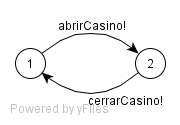
\includegraphics[scale=0.5]{img/admin.png}
\end{center}


{\large FSM: Jugador$_i$}
\begin{center}
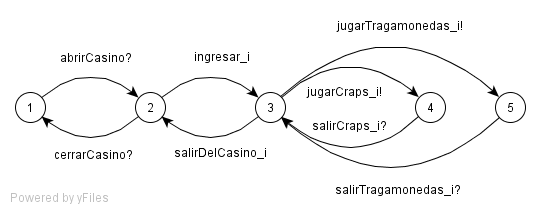
\includegraphics[scale=0.5]{img/jugador.png}
\end{center}

\end{framed}

\subsection{Modo Dirigido}

\subsubsection{Inicio de Modo Dirigido}

Cuando se ingresa en este modo, los resultados de las jugadas no seran al azar sino que el manipulador decidira los mismos.

Esos resultados ingresados se respetaran para todas las jugadas de todas las mesas habilitadas de ese juego mientras no se vuelva a modo normal.

Dicha interaccion con el sistema esta explicada en el caso de uso: \textcolor{red}{falta nombre CU y referencia}

\begin{framed}

\depto Con esta maquina de estados finitos (FSM) Mostramos que en modo dirigido se pueden lanzar jugadas de forma manual, dicha funcionalidad no esta permitida en modo normal.
Es seteo de las jugadas debe hacerse en el momento de entrar en modo dirigido. 

\textcolor{red}{ver orden de las imagenes}

\paragraph{FSM: Administrador}
\begin{center}
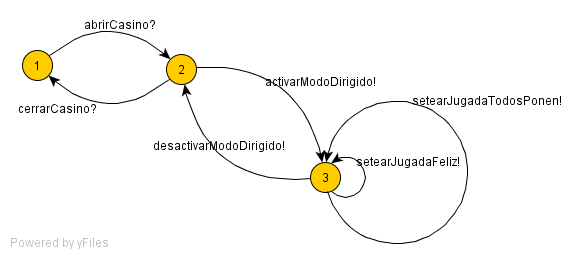
\includegraphics[scale=0.5]{img/manipulador.png}
\end{center}

\end{framed}

\subsubsection{Seteo de Jugadas Feliz y Todos Ponen}

El manipulador puede iniciar una Jugada Feliz, al hacerlo debe seleccionar una unica jugada que se ver� afectada por la Jugada Feliz.

Dicha interaccion con el sistema esta explicada en el caso de uso: \textcolor{red}{falta nombre CU y referencia}

Por otro lado, si el manipulador inicia una Jugada Todos Ponen, al hacerlo puede seleccionar varias jugadas las cuales se veran afectadas (todas) por la jugada de este tipo.

Dicha interaccion con el sistema esta explicada en el caso de uso: \textcolor{red}{falta nombre CU y referencia}

\subsubsection{Finalizaci�n de Modo Dirigido}

En el momento que el manipulador decida abandoanar el modo dirigido, debera desactivarlo.
Y asi volver al modo normal. Ver caso de uso: \textcolor{red}{falta nombre CU y referencia}
                                            
 %asi como la ocurrencia de la jugada feliz y todosponen.


\subsubsection{Pago de una jugada tragamonedas}

\begin{framed}

\depto Notese que una jugada tragamonedas solo tiene una apuesta que resolver.


\lstset{language=ocl}
\lstset{commentstyle=\textit}
\begin{lstlisting}[frame=trbl]{}

-- esta operacion paga la apuesta de una jugada de tragamonedas
-- dicha apuesta tiene que estar activa (de otro modo ya ha sido 
-- pagada) 
-- Se paga la jugada y se cobran los premios correspondientes
pagarJugadaTraga(j:JugadaTragamonedas):void
pre: j.estado = EstadoAp:activa
post: 
  -- pago resultado jugada y pago pozo progresivo 
  --y reseteo pozo progresivo
  pagarJugadaTragaBasica(j)
  -- cobro porcentaje jugada todos ponen
  cobrarJugadaToposPonen(j)
  -- pago jugada feliz y reseteo pozo feliz
  pagarJugadaFeliz(j)
  
  if damePremioTraga(j) <> 0
  then 
    j.estado = EstadoAp:Ganada
  else
    j.estado = EstadoAp:Perdida
    
  j.apuestaTragamonedas.retribucion = 
      j.hechaPor.saldo - j.hechaPor.saldo@pre


-- si la jugada es todos ponen decremento saldo jugador e 
-- incremento pozo feliz
pagarJugadaFeliz(j:JugadaTragamonedas):void
pre:  j.estado = EstadoAp:activa
post:   let tipoJugada = j.tipoDeJugada

  if tipoJugada.oclisTypeOf(Feliz)
    j.hechaPor.saldo = j.hechaPor.saldo@pre + 
        oclAsType(Feliz).pozoFeliz.monto
    oclAsType(Feliz).pozoFeliz.monto = 0
  endif


-- si la jugada es todos ponen decremento saldo 
-- jugador e incremento pozo feliz
cobrarJugadaToposPonen(j:JugadaTragamonedas):void
pre:  j.estado = EstadoAp:activa
post:  let tipoJugada = j.tipoDeJugada

  if tipoJugada.oclisTypeOf(TodosPonen)
  then 
    j.hechaPor.saldo = 

      j.hechaPor.saldo@pre +
      (damePremioTraga(j) + damePremioProgesivo(j)) * 
      100 / oclAsType(TodosPonen).porcentaje
    
    oclAsType(TodosPonen).pozoFeliz.monto = 

      oclAsType(TodosPonen).pozoFeliz.monto@pre + 
      ((damePremioTraga(j) + damePremioProgesivo(j)) * 
      100 / oclAsType(TodosPonen).porcentaje)
      
  endif



-- incremento saldo jugados de jugada y pozo progresivo 
-- (si corresponde)
-- decremento saldo casino
-- decremento pozo (si corresponde)
pagarJugadaTragaBasica(j:JugadaTragamonedas):void
pre:  j.estado = EstadoAp:activa
post:  
  let jornada = Jornada.allInstances->asSecuence->first()

  j.hechaPor.saldo = j.hechaPor.saldo@pre + 
       (damePremioTraga(j) + damePremioProgesivo(j))
  jornada.saldo = jornada.saldo@pre - cualEsElPrepmio(j)
  if damePremioProgesivo(j) <> 0
  then
    PozoProgresivo.allInstances()->asSecuence()->first().monto = 0
  endif


-- devuelve el valor del premio correspondiente a la jugada
damePremioTraga(j:JugadaTagamonesas):Numero
pre:  
post:  let conjRes:Collection  = 
ResultadoPosibleTagamonedas.allInstances()->select(  r |   
            r.res1 = j.res1 and
            r.res2 = j.res2 and
            r.res3 = j.res2 and
            r.cantMonedas = j.apuestaTragamonesas.cantMonedas) 
  let precioFicha = j.mesaTragamonedas.valorFicha

  if not(conjRes->isEmpty()) then
    result = conjRes->asSecuence()->first().ganMonedas * precioFicha 
  else
    result = 0

  endif 


-- devuelve el valor del premio progresivo 
-- correspondiente a la jugada
damePremioProgesivo(j:JugadaTagamonesas):Numero
pre:  true
post:  let conjRes:Collection  = 
ResultadoPosibleTagamonedas.allInstances()->select(r | r.res1 = j.res1 and
            r.res2 = j.res2 and
            r.res3 = j.res2 and
            r.cantMonedas = j.apuestaTragamonesas.cantMonedas) 
  let precioFicha = j.mesaTragamonedas.valorFicha

  if not(conjRes->isEmpty()) then
    if   j.res1 = Fruta::Dinosaurio and
      j.res2 = Fruta::Dinosaurio and
      j.res3 = Fruta::Dinosaurio and
      j.mesaTragamonedas.CantPalancasMax = 3
    then
      result = 
          j.mesaTragamonedas.pozoProgresivo.monto * precioFicha 
    else
      result = 0
    endif
  else
    result = 0
  endif 
  
\end{lstlisting}

\end{framed}



\subsection{JUEGOS: Craps y Tragamonedas}

\subsubsection{Juego Tragamonedas}

Uno de los juegos elegidos por los socios es el \textbf{Tragamonedas}. Las m�quinas tragamonedas juegan con un �nico valor de ficha. Al iniciarse una jugada, el jugador debe abrir una mesa nueva. Al hacerlo debe seleccionar el tipo de ficha con la que se jugara en esa m�quina. La ficha seleccionada debe ser valida; es decir que debe estar entre los valores de ficha del casino.  

En el siguiente Diagrama de actividades se puede observar a grandes rasgos las actividades que realiza un jugador de tragamonedas.

\begin{figure}[h]
	\centering
		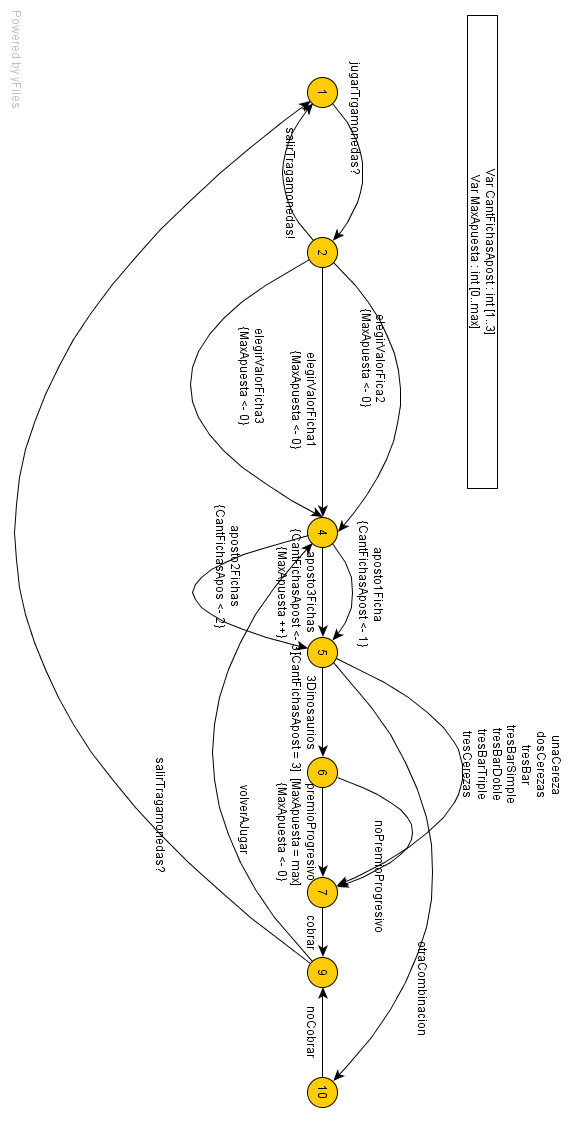
\includegraphics[scale=0.5]{img/JugadorTragamonedas.png}
	\caption{Diagrama de actividades Jugador Tragamonedas\label{fig:JugadorTragamonedas}}
\end{figure}

Cada una de estas actividades se explican con mas detalle en los casos de uso: \textbf{Jugando Tragamonedas} y \textbf{Apostando en tragamonedas}. 
\textcolor{red}{ referencia}


\begin{framed}

\depto Con esta maquina de estados finitos (FSM) mostramos el desarrollo del juego tragamonedas, modelando solo la parte de cobrar o no.

\textcolor{red}{ver orden de las imagenes}

{\large FSM: JugadorTragamonedas}
\begin{center}
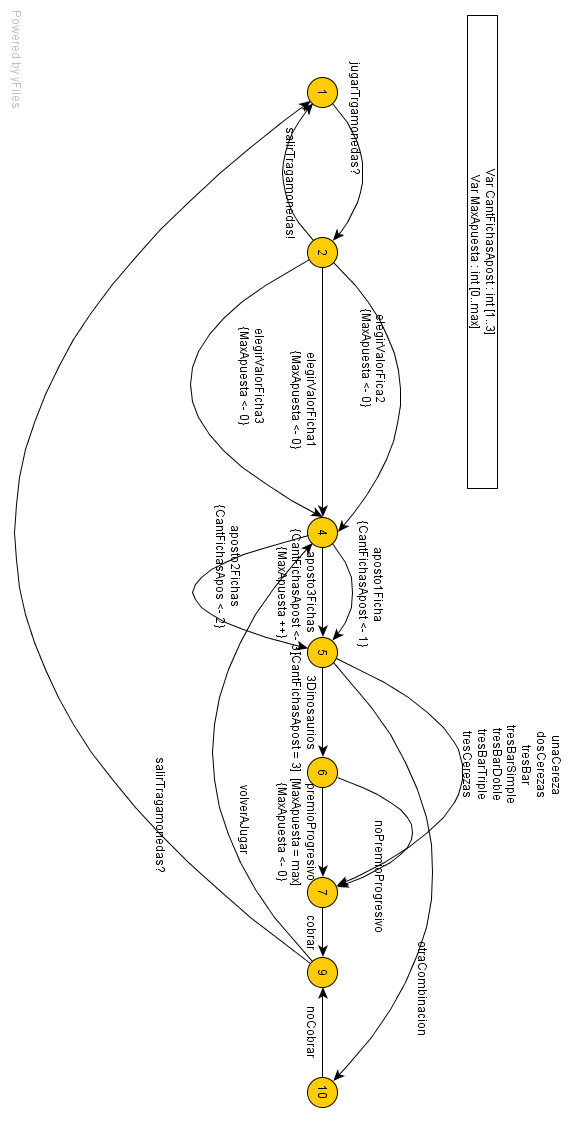
\includegraphics[scale=0.5]{img/JugadorTragamonedas.png}
\end{center}

\end{framed}

Por otro lado, este juego tambien se explica en el modelo conceptual (ver \textcolor{red}{falta referencia} ) con las clases \textcolor{red}{falta poner nombre de las clases}


\subsubsection{CRAPS}

Otro de los juegos elegidos por los socios es el \textbf{Craps}. En este juego un tirador lanza un par de dados para establecer un PUNTO y las apuestas girar�n en base a las posibilidades de que dicho tirador repita el mismo punto antes de lanzar un 7.
Cuando un jugador Craps decida jugar debe seleccionar una mesa existente o abrir una nueva. Luego durante el juego podra tirar los dados y/o apostar.

En el siguiente Diagrama de actividades se puede observar a grandes rasgos las actividades que realiza un jugador de craps.

\begin{figure}[h]
	\centering
		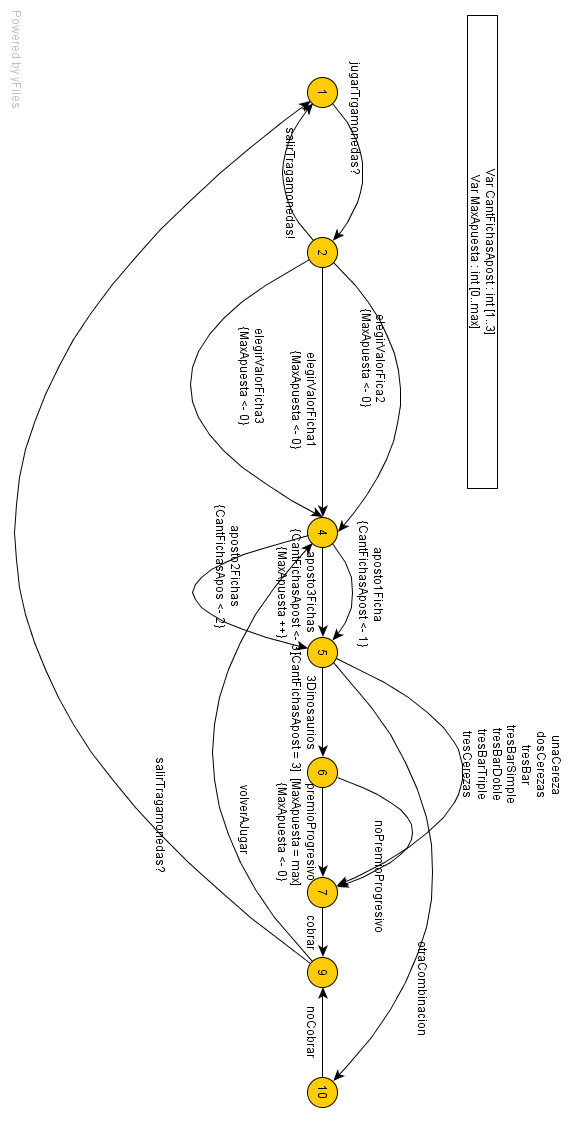
\includegraphics[scale=0.5]{img/JugadorTragamonedas.png}
	\caption{Diagrama de actividades Jugador Tragamonedas\label{fig:JugadorCraps}}
\end{figure}

Cada una de estas actividades se explican con mas detalle en los casos de uso: \textbf{Ingresando a mesa de craps}, \textbf{jugando craps}, apostando craps y \textbf{saliendo mesa craps}. 
\textcolor{red}{ referencia}


\begin{framed}

\depto Con estas maquinas de estados finitos (FSM) mostramos el desarrollo del juego craps. Incluyendo entre ellas un seleccionador, un tirador y cada una de las apuestas. 

\textcolor{red}{ver orden de las imagenes}

{\large FSM: Seleccionador}
\begin{center}
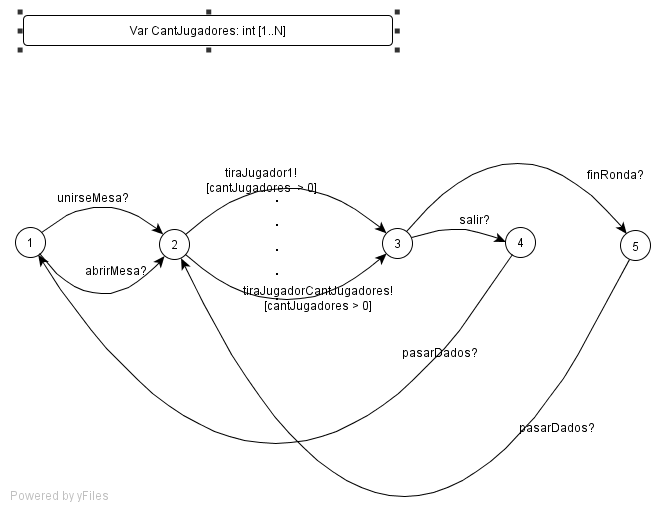
\includegraphics[scale=0.5]{img/seleccionador.png}
\end{center}

{\large FSM: Tirador}
\begin{center}
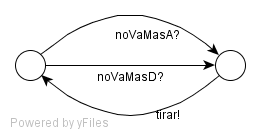
\includegraphics[scale=0.5]{img/tirador.png}
\end{center}

{\large FSM: Desarrollo Craps}
\begin{center}
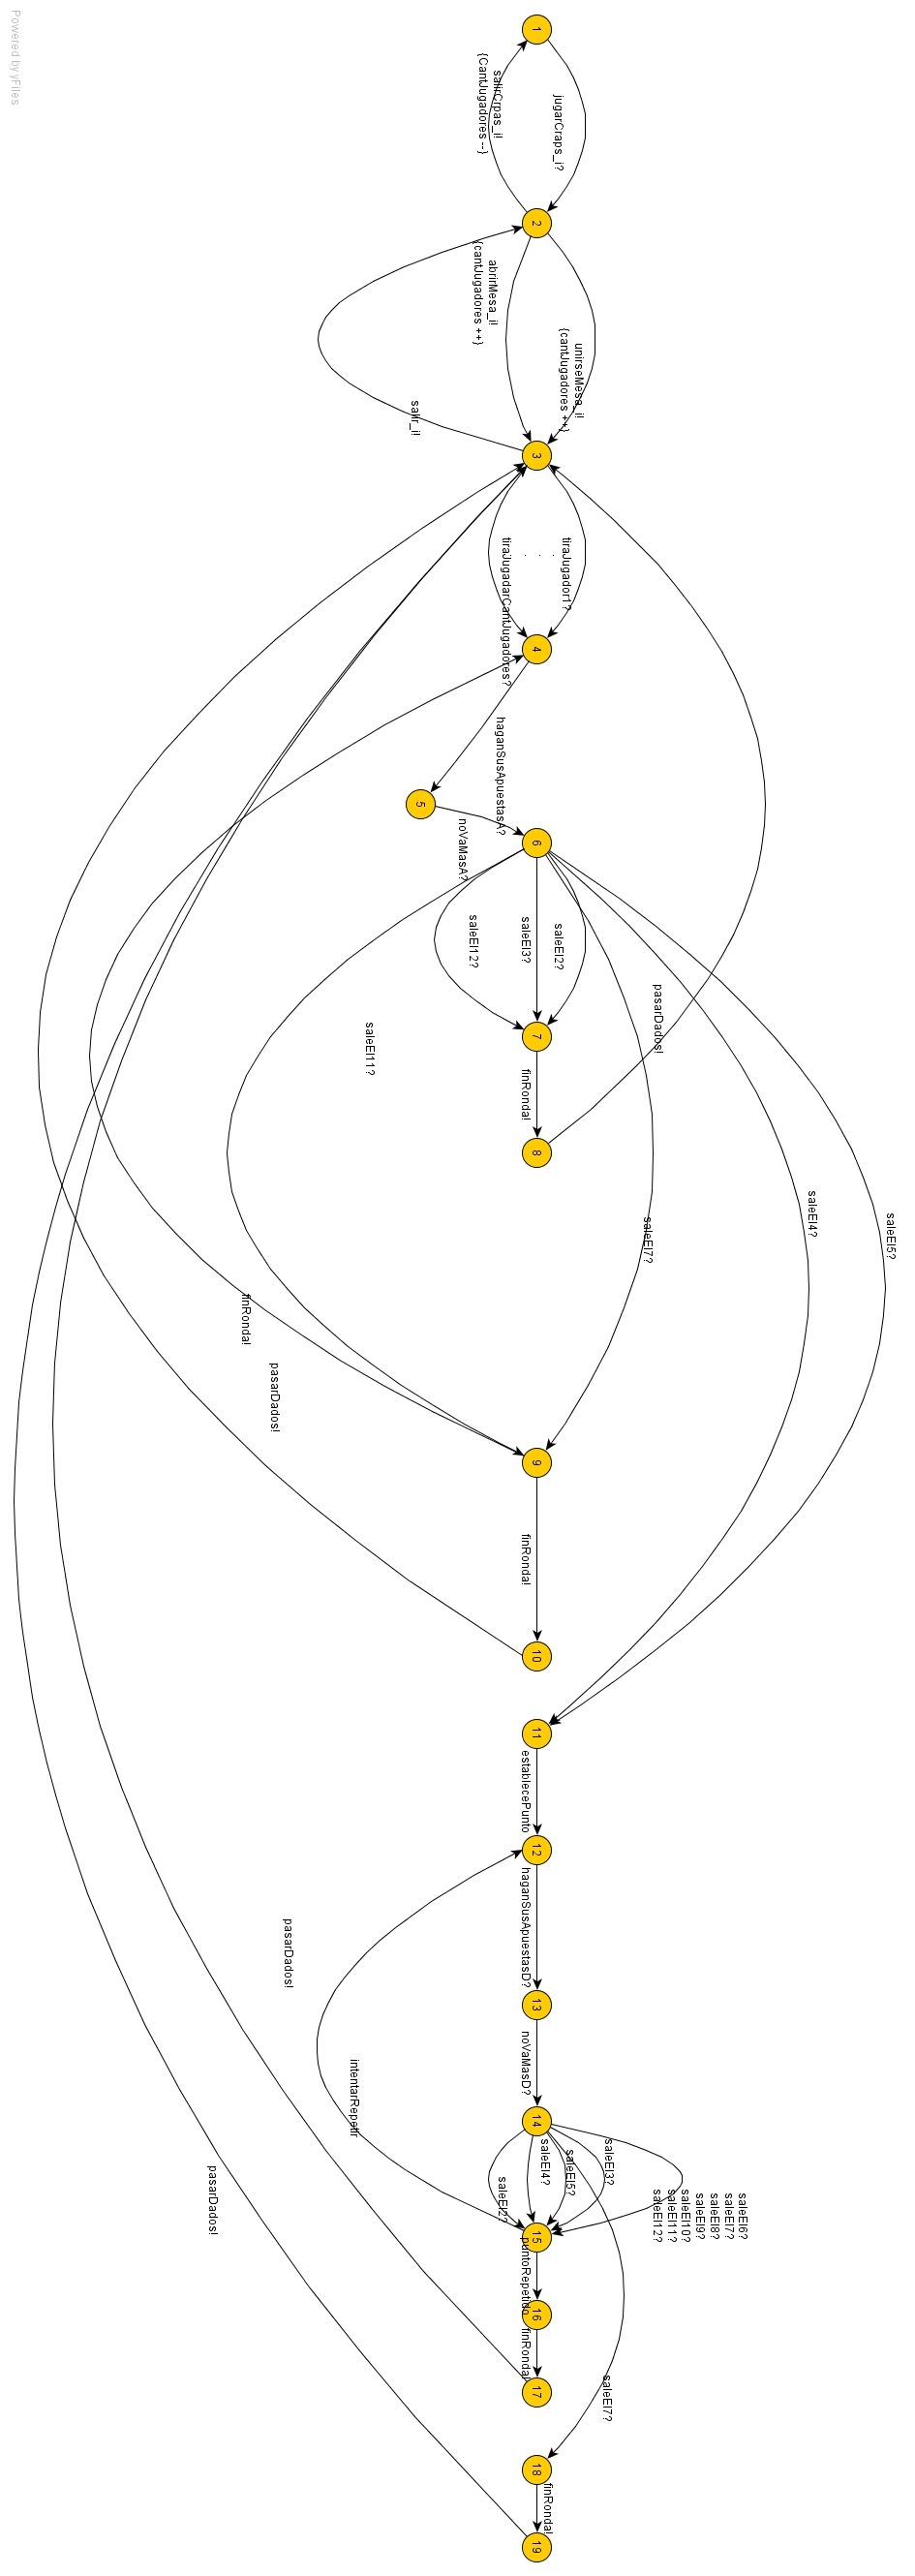
\includegraphics[scale=0.5]{img/desarrolloCraps.png}
\end{center}

Apuestas.

{\large FSM: Linea de Pase}
\begin{center}
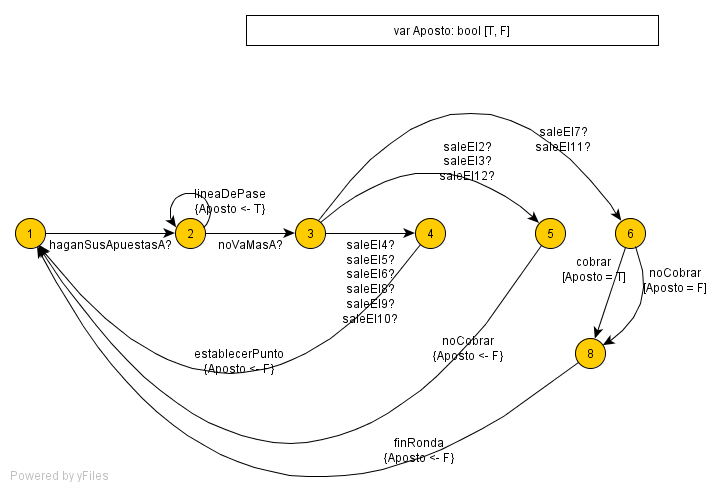
\includegraphics[scale=0.5]{img/linesDePase.png}
\end{center}

{\large FSM: Barra No Pase}
\begin{center}
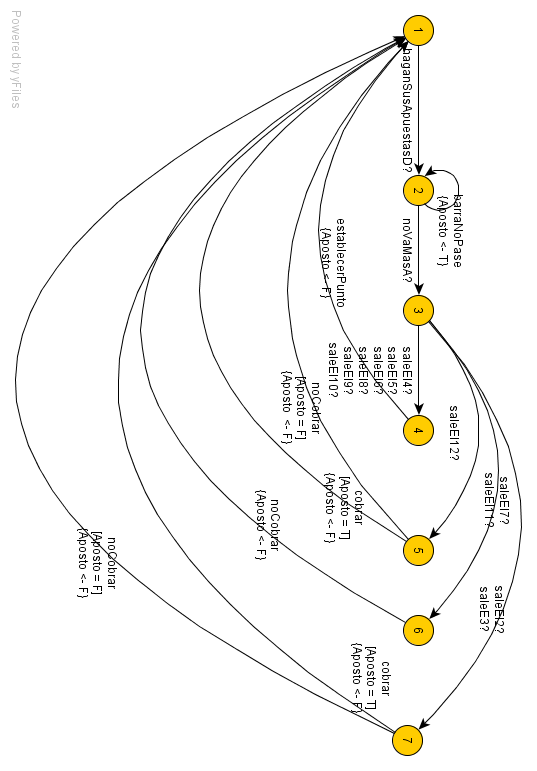
\includegraphics[scale=0.5]{img/barraNoPase.png}
\end{center}



{\large FSM: Apuesta Venir }
\begin{center}
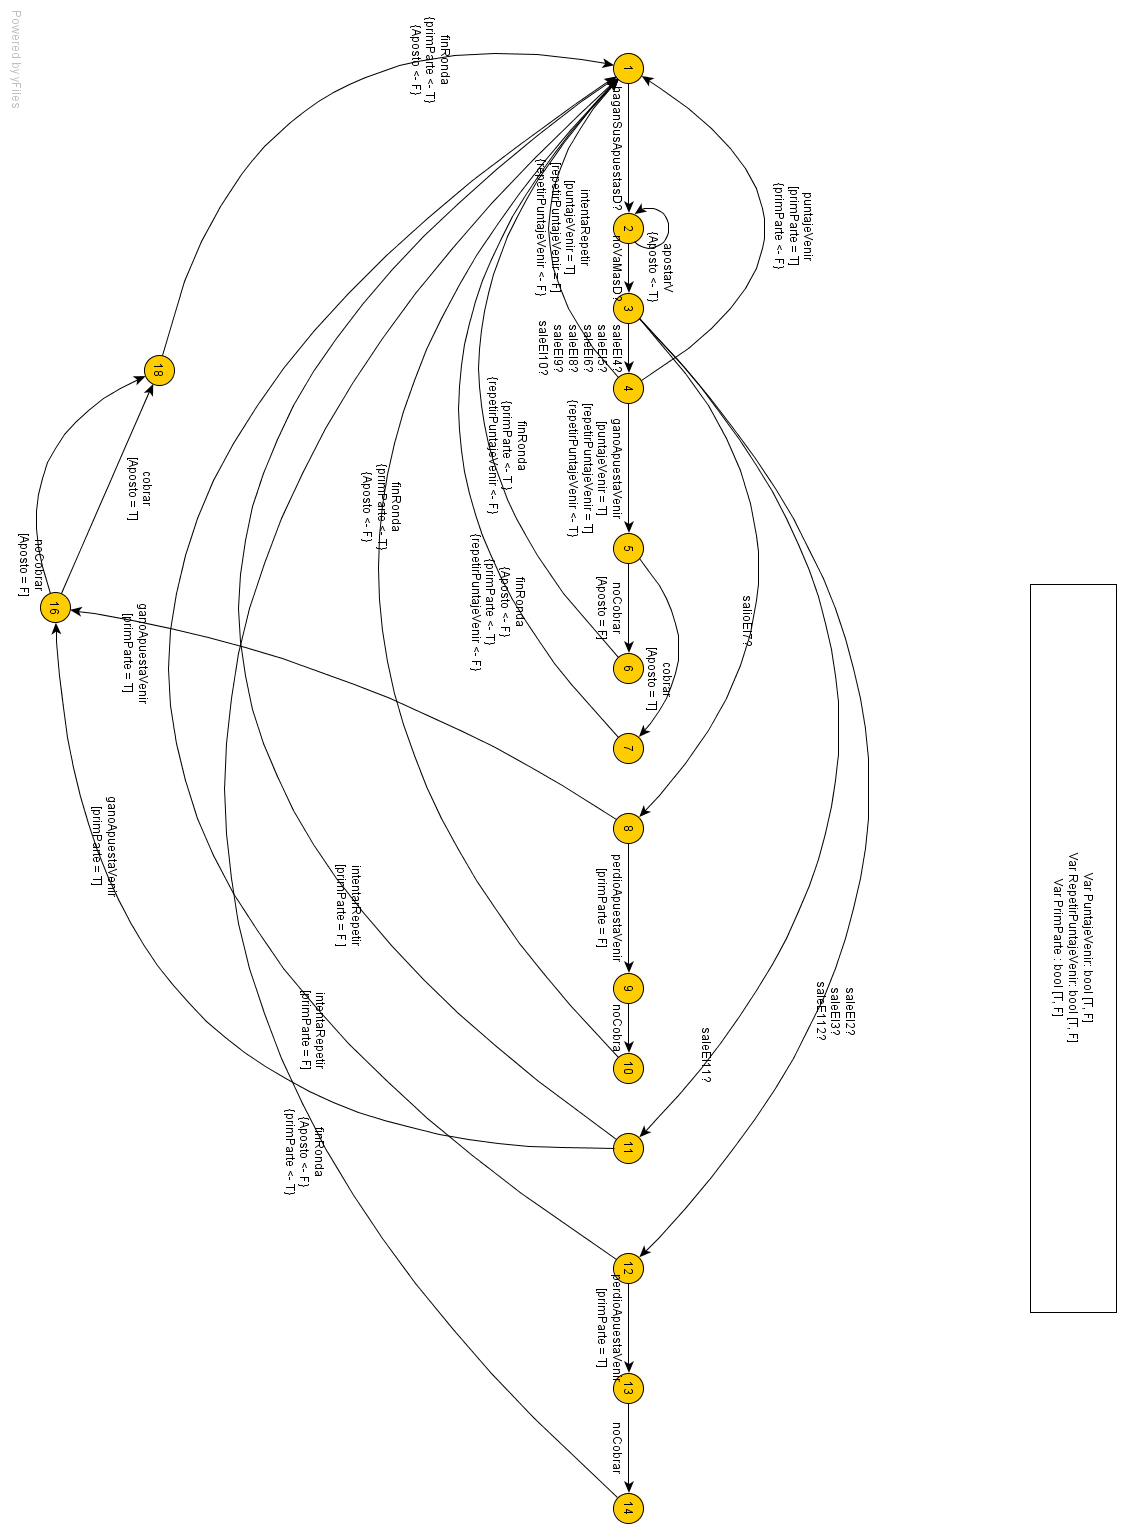
\includegraphics[scale=0.5]{img/ApuestaVenir.png}
\end{center}


{\large FSM: Apuesta No Venir}
\begin{center}
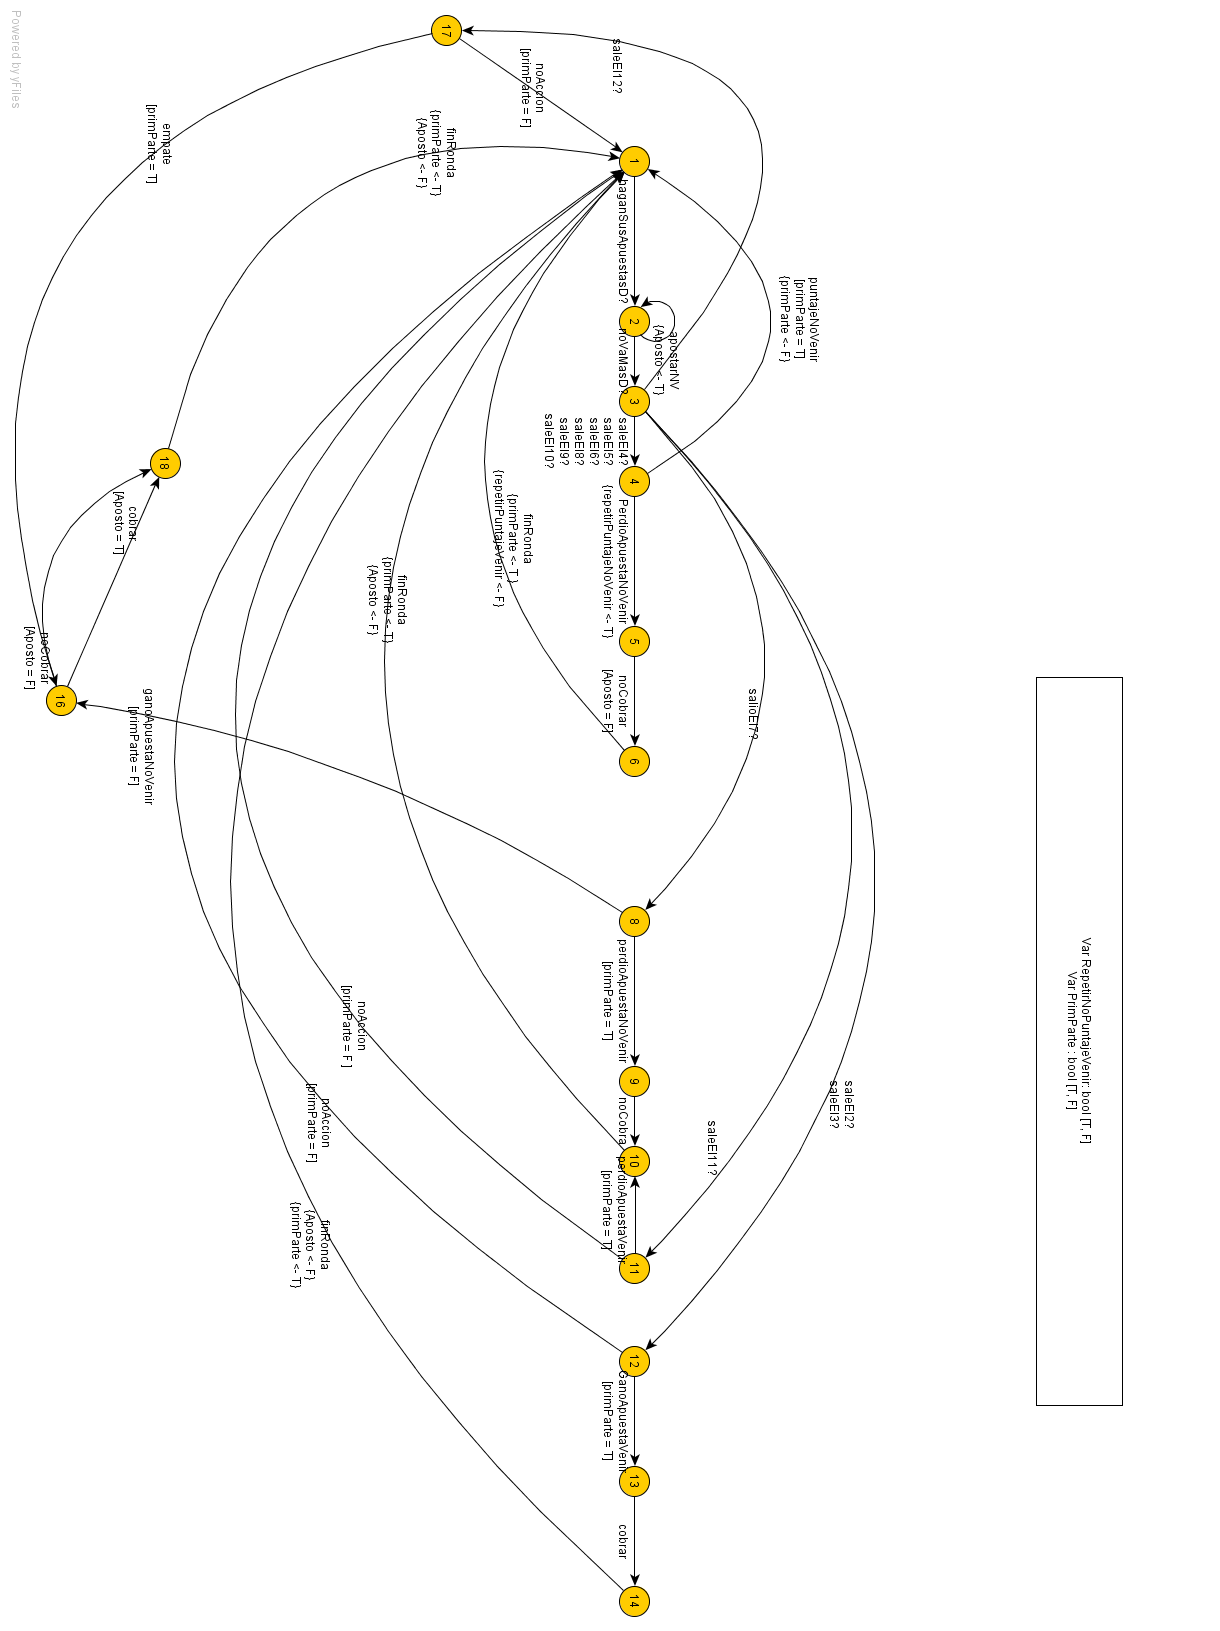
\includegraphics[scale=0.5]{img/apuestaNoVenir.png}
\end{center}


{\large FSM: Apuesta De Campo}
\begin{center}
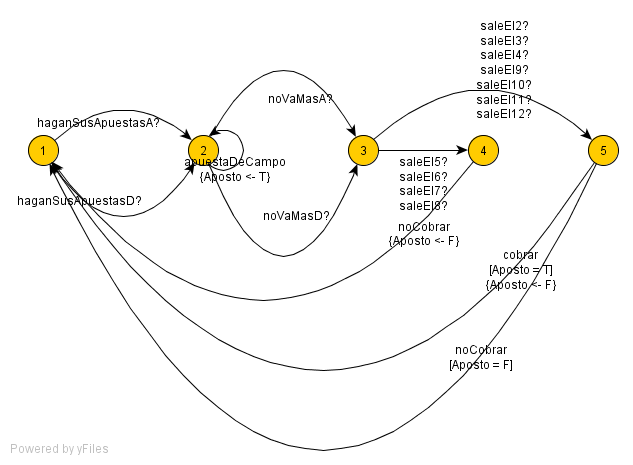
\includegraphics[scale=0.5]{img/apuestaDeCampo.png}
\end{center}

{\large FSM: Apuesta En Sitio}
\begin{center}
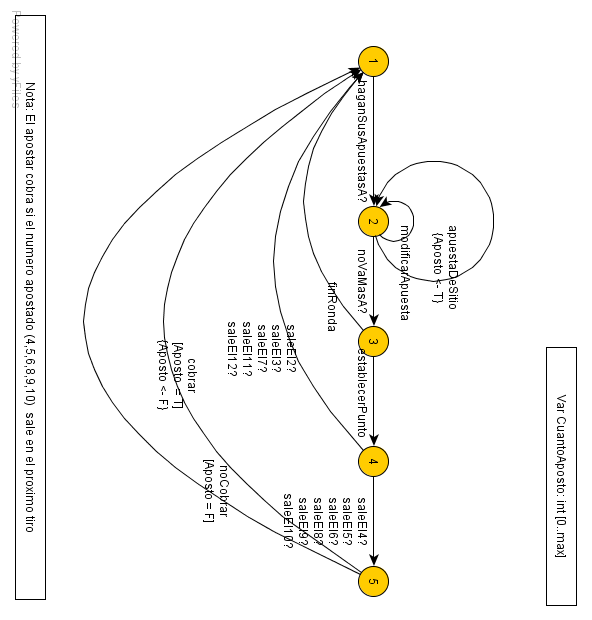
\includegraphics[scale=0.5]{img/apuestaEnSitio.png}
\end{center}


{\large FSM: Apuesta a Ganar}
\begin{center}
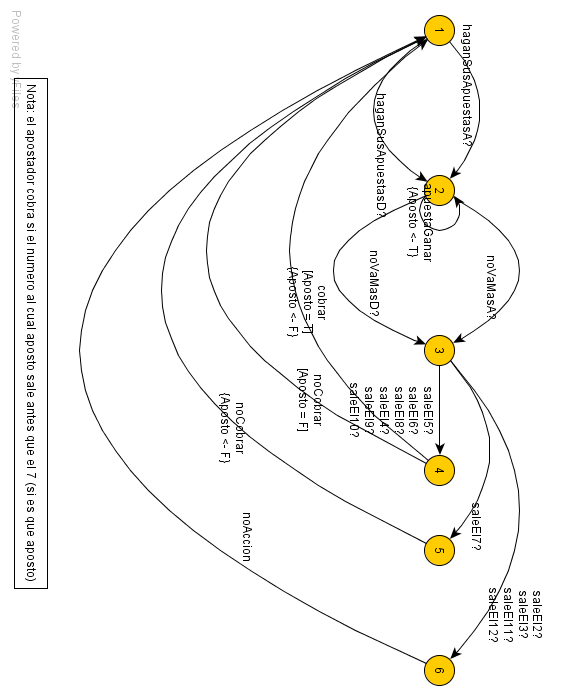
\includegraphics[scale=0.5]{img/apuestaAGanar.png}
\end{center}


{\large FSM: Apuesta En Contra}
\begin{center}
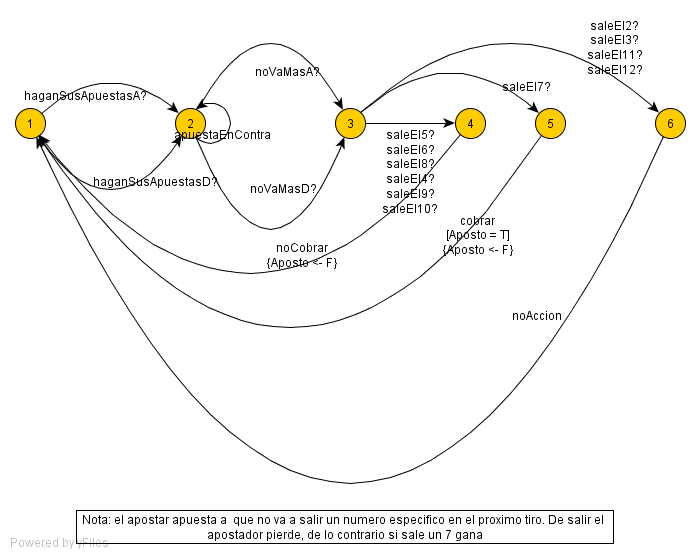
\includegraphics[scale=0.5]{img/apuestaEnContra.png}
\end{center}

\end{framed}

Por otro lado, este juego tambien se explica en el modelo conceptual (ver \textcolor{red}{falta referencia} ) con las clases \textcolor{red}{falta poner nombre de las clases}






















%
%\subsection{Lista de Requerimientos}
%%\newcommand{\ii}{{\bf Importante }}
\newcommand{\ff}{{\bf Funcional }}
\newcommand{\dd}{{\bf Deseable }}
\newcommand{\nd}{{\bf No deseable }}
\newcommand{\nf}{{\bf No funcional }}
\newcommand{\ee}{{\bf Esencial }}

\newcommand{\rrr}{{ \\ \bf REFERIDO EN: }}

\begin{enumerate}

\item\textsc{REQUERIMIENTOS GENERALES DEL CASINO - MANEJO DE CLIENTES}
\begin{enumerate}
\item Los clientes no podr�n apostar mas que el saldo permitido por el departamento de marketing: Los clientes tendr�n un saldo limite y no podr�n realizar ningun tipo de apuesta que sobrepase ese saldo.  \ff - \ii. \rrr \ref{1a1} y en \ref{1a2}
\item Los clientes VIP podr�n apostar ilimitadamente: Los clientes VIP no tiene limite de saldo, por lo tanto no habra ningun monto de apuesta que pueda ser invalidado.  \ff - \ii. \rrr \ref{1b1} y en \ref{1b2}
\item VER Un invitado podr� observar los juegos pero sin participar en ellos: Puede ingresar en una mesa ya abierta y observar el desarrollo del juego pero sin intervenir en el. \ff - \dd. \rrr \ref{1c}
\item Se deber� modificar el saldo del cliente en cada apuesta: Cada vez que un cliente haga una apuesta de cualquier tipo se vera reflejado en la disminuci�n de su saldo.  \ff - \ii. \rrr \ref{1d1} y en \ref{1d2}
\end{enumerate}

\item\textsc{REQUERIMIENTOS GENERALES DEL CASINO - MANEJO DE MESAS}
\begin{enumerate}
\item No se debe permitir que un jugador juegue en mas de una mesa al mismo tiempo: Para ingresar a una mesa de cualquier juego el jugador no podr� estar adentro de ninguna otra mesa de ningun juego.  \ff - \dd. \rrr \ref{2a1} y en \ref{2a2}
\item Los clientes podr�n abrir mesas: Todos los clientes tendran la opci�n de abrir una nueva mesa para cualquiera de los juegos.  \ff - \ee
\item Los clientes podr�n unirse a mesas (s� el juego lo permite): El tragamonedas no permite unirse a una mesa, pero en el Craps el jugador podr� elegir a cual de las mesas habilitadas se unir�.  \ff - \ii
\item Las mesas vacias se cerraran autom�ticamente: Cuando un jugador salga de un juego el sitema autom�ticamente cerrara la mesa a menos que haya otros jugadores en ella.  \ff - \ee
\item El casino no se podr� cerrar mientras haya gente jugando: El casino solo podr� cerrar cuando todos los jugadores hayan salido del mismo.  \ff - \ii
\item No debe haber limite de mesas abiertas: Los clientes podr�n ingresar a las mesas de los juegos y no habra un limite de ellas.  \ff - \ii
\end{enumerate}

\item\textsc{REQUERIMIENTOS GENERALES DEL CASINO - PANTALLA}
\begin{enumerate}
\item Las pantallas mostraran la informaci�n necesaria para el desarrollo del juego: Las pantallas mostrar�n la interfaz del juego asi como tambien todas las opciones disponibles dentro del juego.  \ff - \ii
\item Las pantallas mostraran la informaci�n necesaria del estado del juego: Las pantallas mostraran el tipo de jugada, estado actual del juego y resultados, y ser� inmediatamente actualizada ante cualquier cambio o variaci�n.  \ff - \ii
\item Las pantallas mostraran el estado de la cuenta del jugador: Por pantalla se podr� ver si un jugador esta dentro del casino y dentro de algun juego y si es as� en que mesa, si ha resultado ganador o no, y su correspondiente saldo.  \ff - \dd
\end{enumerate}

\item\textsc{REQUERIMIENTOS GENERALES DEL CASINO - CONFIGURACION}
\begin{enumerate}
\item Permitir la configuraci�n est�tica del monto m�nimo de los pozos: Se podr� permitir configurar el monto minimo que debe superar un pozo antes de poder entregarlo.  \nf - \dd
\end{enumerate}

\item\textsc{REQUERIMIENTOS GENERALES DEL CASINO - FICHAS}
\begin{enumerate}
\item Las apuestas se har�n por medio de fichas: En todos los juegos el jugador podr� elegir el monto a apostar seleccionando de entre los valores establecidos de las fichas.  \ff - \ii
\item Las fichas ser�n ilimitadas: No habra una cantidad fija de fichas sino que se dispondr� de ellas en un numero ilimitado.  \ff - \ii
\item El valor de las fichas debe poder configurarse por el administrador: Cada vez que el casino abre al administrador configurara los valores posibles de las fichas.  \nf - \ii
\end{enumerate}

\item\textsc{REQUERIMIENTOS GENERALES DEL CASINO - REPORTES}
\begin{enumerate}
\item Generar informe electr�nico: Ranking de jugadores: Se generar� un informe con los jugadores que m�s dinero ganaron en el d�a desde que abrio el casino, como tambi�n los que m�s dinero perdieron. \ff - \ii
\item Generar informe electronico: Estado Actual: Se generar� un informe con el estado del casino y su saldo y tambi�n el de los clientes. \ff - \ii
\item Generar informe electronico: Detalle de movimientos por jugador: Se generar� un informe con todas las apuestas, premios ganados, y montos ganados por cada jugador que haya ingresado al casino. \ff - \ii
\end{enumerate}

\item\textsc{REQUERIMIENTOS GENERALES DEL CASINO - JUGADAS Y POZOS}
\begin{enumerate}
\item Mostrar en todo momento el monto de los pozos: En todo momento se mostrara el monto actualizado de todos los pozos del casino, y se actualizar� inmediatamente a medida que varie. \ff - \ii
\item Generar jugada feliz autom�ticamente: La jugada feliz se generara en base a probabilidades.  \ff - \ee
\item Generar jugada todos ponen autom�ticamente: La jugada todos ponen tambien se generara en base a probabilidades.  \ff - \ee
\item No se debe permitir el solapamiento de jugadas felices en el mismo instante: Si ha ocurrido una, entonces no podra ocurrir otra hasta que se pague la jugada existente y se supere el monto minimo, aunque pueden ocurrir en cualquiera de las mesas del casino pero no simultaneamente.  \ff - \ii
\end{enumerate}

\item\textsc{REQUERIMIENTOS GENERALES DEL CASINO - MODO DIRIGIDO}
\begin{enumerate}
\item El sistema deber� contar con un modo dirigido: Se podra poner en modo dirigido a cada uno de los juegos y todas sus respectivas mesas tendr�n como resultado el definido por el manipulador de modos.  \ff - \ii
\item El sistema deber� permitir generar jugada feliz manualmente: El manipulador de modos podr� decidir la ocurrencia de jugadas felices mientras no se solapen simultaneamente en los juegos del casino.  \ff - \ii
\item El sistema deber� permitir generar jugada todos ponen manualmente: El manipulador de modos podr� decidir la ocurrencia de jugadas todos ponen mientras no se solapen en la misma jugada. \ff - \ii
\end{enumerate}

\item\textsc{REQUERIMIENTOS DE JUEGO TRAGAMONEDAS}
\begin{enumerate}
\item Proveer juego Tragamonedas: Se proveera el juego del Tragamonedas respetando las reglas provistas por los clientes.  \ff - \ee. \rrr \ref{9a}
\item El juego Tragamonedas debe contar con un premio gordo progresivo: El juego de Tragamonedas permitira incrementar el premio gordo progresivo usando un porcentaje de cada una de las jugadas para ser otorgado luego de superar el monto minimo configurado al que obtenga la combinacion ganadora y haya apostado las n veces anteriores al maximo numero de fichas. \ff - \ee. \rrr \ref{9b}
\item El cliente podr� elegir entre varios valores de fichas de las maquinas tragamonedas: Se podr� elegir una mesa de maquina tragamonedas de distintos valores entre los definidos. Una vez elegido el valor de la ficha para el tragamonedas este no se podr� cambiar hasta salir del juego.  \ff - \nd. \rrr \ref{9c}
\end{enumerate}

\item\textsc{REQUERIMIENTOS DE JUEGO CRAPS}
\begin{enumerate}
\item Proveer juego Craps: Se proveera el juego de Craps respetando las reglas provistas por los clientes. \ff - \ee. \rrr \ref{10a}
\end{enumerate}

\item\textsc{REQUERIMIENTOS DE IMPLEMENTACION Y COMPORTAMIENTO}
\begin{enumerate}
\item El sistema debe funcionar en red.  \nf - \ee
\item VER El sistema a implementarse deber� estar realizado en Java o C$\#$ \nf - \ii 
\item VER El sistema debe ser facilmente extendible con nuevos juegos \nf - \ii 
\end{enumerate}


\item\textsc{REQUERIMIENTOS DE FUNCIONALIDAD EXTRA}
\begin{enumerate}
\item VER Se podr�n ver imagenes de los juegos en 3D \ff - \dd
\item VER Los jugadores podran chatear entre ellos dentro del juego \ff - \dd
\end{enumerate}

\end{enumerate}



%
%\subsection{Diagrama de contexto}
%
%Ilustraremos los fenomenos esenciales entre los distintos \agentes involucrados, el \dominio de todo el \sistema y el \alcance del software a desarrollar.
%
%\begin{figure}[htp]
%    \centering
%		\includegraphics[scale=0.5]{dc.png}
%	\caption{Diagrama de contexto \label{fig:dc}}
%\end{figure}
%
%\paragraph{Nota:}
%Como vemos en la figura: \ref{fig:dc} el manejo de registracion y administracion del dinero real queda fuera del alcanze del software, este solamente recibira un archivo por parte del administrador y trabajar� sobre dicha informacion.
%
%\subsection{Diagrama de Objetivos}
%
%\begin{figure}[htp]
%	\centering
%		\includegraphics[scale=0.3, angle=90]{do.png}
%	\caption{Diagrama de Objetivos \label{fig:do}}
%\end{figure}
%
%\subsection{Casos de Uso}
%%%%%%%%ACTORES
%%%%%%\newcommand{\pc}{{\bf Cliente del casino }}
%%%%%%\newcommand{\adm}{{\bf Administrador }}
%%%%%%%\newcommand{\ptra}{{\bf Potencial jugador de tragamonedas }}
%%%%%%\newcommand{\jutra}{{\bf Jugador de Tragamonedas }}
%%%%%%\newcommand{\jc}{{\bf Jugador de Craps }}
%%%%%%\newcommand{\jac}{{\bf Apostador de Craps }}
%%%%%%\newcommand{\emc}{{\bf Empleado Contable }}
%%%%%%\newcommand{\emk}{{\bf Empleado de Marketing }}
%%%%%%\newcommand{\aptra}{{\bf Apostador de Tragamonedas }}
%%%%%%\newcommand{\apocr}{{\bf Apostador de Craps }}
%%%%%%\newcommand{\jucr}{{\bf Potencial Jugador de Craps }}
%%%%%%%CASOS DE USO
%%%%%%\newcommand{\ic}{{\bf Ingresando a casino }}
%%%%%%\newcommand{\salc}{{\bf Saliendo del casino }}
%%%%%%\newcommand{\atra}{{\bf Abriendo Mesa Tragamonedas }}
%%%%%%\newcommand{\jtra}{{\bf Jugando Tragamonedas }}
%%%%%%\newcommand{\actm}{{\bf Activando Modo Dirigido }}
%%%%%%\newcommand{\desm}{{\bf Desactivando Modo Dirigido }}
%%%%%%\newcommand{\jugf}{{\bf Jugada Feliz }}
%%%%%%\newcommand{\jugtp}{{\bf Jugada Todos Ponen }}
%%%%%%\newcommand{\ac}{{\bf Abriendo Casino }}
%%%%%%\newcommand{\cc}{{\bf Cerando Casino }}
%%%%%%\newcommand{\apotra}{{\bf Apostando en Tragamonedas }}
%%%%%%\newcommand{\incr}{{\bf Ingresando a mesa de Craps }}
%%%%%%\newcommand{\scr}{{\bf Saliendo de mesa de Craps }}
%%%%%%\newcommand{\jcr}{{\bf Jugando Craps }}
%%%%%%\newcommand{\apcr}{{\bf Apostando Craps }}
%%%%%%\newcommand{\admin}{{\bf administrador}}
%%%%%%\newcommand{\ccas}{{\bf Cerrando Casino}}
%%%%%%\newcommand{\empmark}{{\bf Empleado de Marketing}}
%%%%%%\newcommand{\infomovjug}{{\bf Pidiendo informes}}
%%%%%%\newcommand{\infoestact}{{\bf informe Estado Actual}}
%%%%%%\newcommand{\inforankjug}{{\bf informe Ranking de Jugadores}}
%%%%%%\newcommand{\infdmj}{{\bf Pidiendo informe Detalles de movimientos por jugador}}
%%%%%%\newcommand{\infea}{{\bf Pidiendo informe Estado Actual}}
%%%%%%\newcommand{\infrj}{{\bf Pidiendo informe Ranking de Jugadores}}


\newcommand{\req}{{\bf Requerimientos satisfechos por este Caso de Uso: }}
%ACTORES
\newcommand{\pc}{{\bf Cliente del casino }}
\newcommand{\adm}{{\bf Administrador }}
\newcommand{\invi}{{\bf Invitado }}
%\newcommand{\ptra}{{\bf Potencial jugador de tragamonedas }}
\newcommand{\jutra}{{\bf Jugador de Tragamonedas }}
\newcommand{\pjc}{{\bf Potencial jugador de Craps }}
\newcommand{\jc}{{\bf Jugador de Craps }}
\newcommand{\apcr}{{\bf Apostador de Craps }}
\newcommand{\emc}{{\bf Empleado Contable }}
\newcommand{\emk}{{\bf Empleado de Marketing }}
\newcommand{\jucr}{{\bf Tirador de Craps}}
\newcommand{\mani}{{\bf Manipulador }}
%CASOS DE USO
\newcommand{\ic}{{\bf Ingresando al casino }}
\newcommand{\salc}{{\bf Saliendo del casino }}
\newcommand{\inginvi}{{\bf Ingresando al casino como invitado}}
\newcommand{\salinvi}{{\bf Saliendo del casino como invitado }}
\newcommand{\obser}{{\bf Observando Juego }}
\newcommand{\intr}{{\bf Ingresando a mesa de Tragamonedas }}
\newcommand{\jtra}{{\bf Jugando Tragamonedas }}
\newcommand{\satr}{{\bf Saliendo a mesa de Tragamonedas }}
\newcommand{\incr}{{\bf Ingresando a mesa de Craps }}
\newcommand{\jugcr}{{\bf Jugando Craps }}
\newcommand{\apocr}{{\bf Apostando Craps }}
\newcommand{\sacr}{{\bf Saliendo a mesa de Craps }}
\newcommand{\actm}{{\bf Activando Modo Dirigido }}
\newcommand{\desm}{{\bf Desactivando Modo Dirigido }}
\newcommand{\jugf}{{\bf Iniciando Jugada Feliz Manipulada}}
\newcommand{\jugtp}{{\bf Iniciando Jugada Todos Ponen Manipulada}}
\newcommand{\ac}{{\bf Abriendo Casino }}
\newcommand{\cc}{{\bf Cerrando Casino }}
\newcommand{\infdmj}{{\bf Pidiendo informe Detalles de movimientos por jugador}}
\newcommand{\infea}{{\bf Pidiendo informe Estado Actual}}
\newcommand{\infrj}{{\bf Pidiendo informe Ranking de Jugadores}}  %FALTA poco
